\documentclass[12pt,a4paper]{article}
%\usepackage[in]{fullpage}
\usepackage[utf8x]{inputenc}
\usepackage{cite}
%\usepackage{listings}
\usepackage[usenames]{xcolor}
\usepackage{graphicx}
\usepackage{hyperref}
\usepackage{float} %for H positioning
%\usepackage[backend=bibtex]{biblatex}
%\addbibresource{references.bib}

%\lstset{ %
%  basicstyle=\footnotesize,        % the size of the fonts that are used for the code
%  breakatwhitespace=true,          % sets if automatic breaks should only happen at whitespace
%  breaklines=true,                 % sets automatic line breaking
%  commentstyle=\color{gray},    % comment style
%  keepspaces=true,                 % keeps spaces in text, useful for keeping indentation of code (possibly needs columns=flexible)
%  language=bash                 % the language of the code
%}

% latest version of the mrfioc2 device support
\newcommand{\latestDriverVersion}{2.7.9}

%opening
\title{EVR Tutorials}
%\author{Sašo Skube, PSI}
\date{}

\begin{document}



\maketitle

\tableofcontents
\newpage

\section{Introduction}
A timing system consists of an event generator (EVG), a series of event receivers (EVR), software controlling them and a timing network. EVG generates a series of events, which are delivered to EVRs through a timing network. An EVR is then configured to respond to specific events in various ways, including processing EPICS records and generating pulses, synchronized clock or custom signals on its outputs.
This document contains step-by-step instructions to configuring some of the basic functionalities of the event receiver. A detailed EVR manual is available in~\cite{evr_manual}.

\section{Quick start}\label{sec:Quick start}
To set up a timing system we need a VME crate, a Single Board Computer (SBC) and an EVR. A VME crate has a number of slots where SBC, EVR and other components can be inserted. Slot numbering should be checked with the VME crate documentation. The tutorials in this document are written for the following setup:
\begin{itemize}
	\item a VME64x IFC 1210 Single Board Computer inserted into VME crate slot 1 (how to set up IFC 1210~\cite{ifc}),
	\item EVR-VME-230RF event receiver inserted in slot 3,
	\item the EVR connected to the timing network through an optical cable.
\end{itemize}

To set up an IOC application for EVR we need to set up a startup script and a substitution file. Suitable ones are available in the mrfioc2 git repository~\cite{git_mrfioc2}, under the \texttt{PSI/example} folder.

The following steps demonstrate how to prepare a SWIT compatible IOC application that utilizes EVR:
\begin{enumerate}

	\item Create a project folder, eg. \texttt{MTEST-VME-TIMINGTEST} and a sub-folder named \texttt{cfg} in your project folder: \texttt{MTEST-VME-TIMINGTEST/cfg/}
\begin{verbatim}
	mkdir MTEST-VME-TIMINGTEST
	cd MTEST-VME-TIMINGTEST
	mkdir cfg
\end{verbatim}

	\item Create a substitution file for your project (can be empty), named \texttt{MTEST-VME-TIMINGTEST\_main.subs} using the following command: 
\begin{verbatim}
	touch MTEST-VME-TIMINGTEST_main.subs
\end{verbatim}	
	This substitution file can be used to load custom templates, but it must be present in order for SWIT~\cite{swit} to work properly.
	
	\item 
		Create a substitution file named \texttt{EVR0.subs} in your project's \texttt{cfg} sub-folder:
		\begin{verbatim}
			cd cfg
			touch EVR0.subs
			cd ..
		\end{verbatim}
	\item \label{quickstart:copySubs} Copy the content of the substitution file  at \texttt{https://git.psi.ch/} \texttt{epics\_drivers/mrfioc2/raw/\latestDriverVersion/PSI/example/evr\_VME-230.subs} to newly created \texttt{cfg/EVR0.subs}. This substitution file can always be used as a starting point for new applications. Substitution files for other form factors are available at the same location (mrfioc2 repository in folder \texttt{PSI/example}).
	
	The macro definitions in the substitution file are used to configure the EVR. All the available macros are already present in the substitution file and set to their default values, so the user can simply change the desired values. Detailed description of the substitution file is available in the EVR manual~\cite{evr_manual}.

	\item
		Create a startup script named \texttt{MTEST-VME-TIMINGTEST\_startup.script} in your project folder:
		\begin{verbatim}
			touch MTEST-VME-TIMINGTEST_startup.script
		\end{verbatim}
	\item 
		Copy the content of the startup script at \texttt{https://github.psi.ch/projects/} \texttt{ED/repos/mrfioc2/browse/PSI/example/evr\_VME\_startup.script?at=\latestDriverVersion} to newly created \texttt{MTEST-VME-TIMINGTEST\_startup.script}. Startup scripts for other form factors are available at the same location (mrfioc2 repository in folder \texttt{PSI/example}).

	The startup script should look similar to:
\begin{verbatim}
	require mrfioc2
	
	##########################
	#-----! EVR Setup ------!#
	##########################
	## The following parameters are available to set up the device. 
	## They can either be set as an epics environmental variable, 
	## or passed as a macro to the 'runScript' command:
	
	# The following macros are available to set up the mrfioc2:
	# SYS           "MTEST-VME-TIMINGTEST"
	# DEVICE        "EVR0"		
	# EVR_SLOT		     3			
	# EVR_MEMOFFSET	0x3000000
	# EVR_IRQLINE 	 0x5		
	# EVR_IRQVECT	  0x26
	# EVR_SUBS      cfg/evr_VME-300.subs
	
	runScript $(mrfioc2_DIR)/mrfioc2_evr-VME.cmd, 
	  "SYS=MTEST-VME-TIMINGTEST, DEVICE=EVR0, EVR_SLOT=3,
	   EVR_MEMOFFSET=0x3000000, EVR_IRQLINE=0x5"
\end{verbatim}
Startup script overview:
\begin{itemize}
\item 
	\texttt{require mrfioc2} loads the mrfioc2 module. More information about \texttt{require} command is available at driver.makefile wiki page~\cite{driver.makefile}.
\item 
	A few comments that serve as a quick documentation, describing available variables which user can set.
\item 
	\texttt{runScript} command is issued. It initializes the mrfioc2 device support and loads appropriate substitution files. It accepts a number of configurable variables. More information about \texttt{runScript} command is available at driver.makefile wiki page~\cite{driver.makefile}.
\end{itemize}

The configurable variables in the startup script are:
\begin{itemize}
	\item
		\texttt{SYS} is the system name. \textbf{This variable is mandatory.}
	\item 
		\texttt{DEVICE} is the event receiver / timing card name. If the variable is not defined in the startup script, it defaults to \texttt{EVR0}.
	\item 
		\texttt{EVR\_SLOT} is the VME crate slot where EVR is inserted. If the variable is not defined in the startup script, it defaults to \texttt{3}.
	\item 
		The base A32 address (\texttt{EVR\_MEMOFFSET}), interrupt level (\texttt{EVR\_IRQLINE}) and interrupt vector (\texttt{EVR\_IRQVECT}) variables configure the interaction between the SBC and the EVR. The details are out of scope of this document. If a variable is not defined in the startup script, it gets set to its default value. Default values are:
		\begin{itemize}
		\item \texttt{EVR\_MEMOFFSET} = 0x3000000
		\item \texttt{EVR\_IRQLINE} = 0x5
		\item \texttt{EVR\_IRQVECT} = 0x26
		\end{itemize}
	\item 
		\texttt{EVR\_SUBS} is the substitution file that we are using for our application. If not specified, a substitution file in \texttt{cfg/\$(EVR).subs} (where \$(EVR) is the event receiver name) will be loaded.
\end{itemize}
Using the above startup script, the system name is set to \textit{MTEST-VME-TIMINGTEST}, and the event receiver named \textit{EVR0} is placed in the physical slot 3 of the VME crate. It uses default A32 address and interrupt configuration. Substitution file \texttt{cfg/EVR0.subs} will be loaded.
\end{enumerate}


\section{Generate a pulse upon receiving an event}
EVR has a number of pulsers available and each of them can generate a pulse upon receiving an event. The pulse can then be outputted through desired EVR outputs. 

This tutorial demonstrates how to configure an EVR to generate a 80 ns wide pulse, 40 ns after each reception of event 4, as seen in Figure~\ref{fig:pulser_signal}. 
\begin{figure}[H]
	\centering
	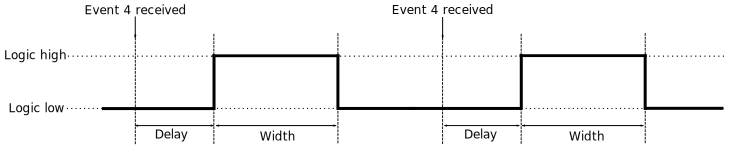
\includegraphics[width=\columnwidth]{./img/pulserSignal}
	\caption{An example of a pulse generated after the reception of the event 4.}
	\label{fig:pulser_signal}
\end{figure}
The pulse in this tutorial is generated using pulser 3 and outputted through the front panel TTL output 0 (FrontOut0), as seen in Figure~\ref{fig:pulser}. 

\begin{figure}[H]
	\centering
	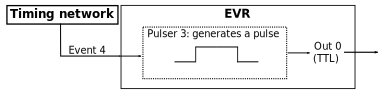
\includegraphics[]{./img/pulser}
	\caption{Use pulser 3 to generate a pulse upon reception of the event 4. The pulse is outputted through front panel TTL output 0.}
	\label{fig:pulser}
\end{figure}

\subsection{Instructions}
\begin{enumerate}
	\item If starting a new IOC application, consult the quick start in Section~\ref{sec:Quick start}.

	\item Set the macro values in the substitution file (\texttt{MTEST-VME-TIMINGTEST/} \texttt{cfg/EVR0.subs}) according to this snippet (explained in~\ref{sec:explain_pulser}):
\begin{verbatim}
	file "$(mrfioc2_TEMPLATES=db)/evr-vme-230.db"
	{
	  {
	    ...
	    Pul3-Delay-SP=40,
	    Pul3-Width-SP=80,
	    ...
	    FrontOut0-Src-SP=3,
	    ...
	  }
	}

	file "$(mrfioc2_TEMPLATES=db)/evr-pulserMap.template"{
	pattern { PID   F,       EVT, ID}
	        ...
	        { 3,    Trig,    4,   0 }
	        ...
	}
\end{verbatim}
	The above macro substitution of the \texttt{evr-vme-230.db} sets the values of the following records:
	\begin{itemize}
	\item \texttt{MTEST-VME-TIMINGTEST-EVR0:Pul3-Delay-SP}
	\item \texttt{MTEST-VME-TIMINGTEST-EVR0:Pul3-Width-SP}
	\item \texttt{MTEST-VME-TIMINGTEST-EVR0:FrontOut0-Src-SP}
	\end{itemize}
	The above macro substitution of the \texttt{evr-pulserMap.template} creates a record named \texttt{MTEST-VME-TIMINGTEST-EVR0:Pul\$(PID)-Evt-\$(F)\$(ID)-SP}.
	\item Optionally, you can remove all the macros whose values you did not change. 
	\item Install the prepared IOC by running command \texttt{swit -V} from your project folder \textit{MTEST-VME-TIMINGTEST}.
\end{enumerate}
\subsection{Substitution snippet explanation:}\label{sec:explain_pulser}

First we set up the pulse generator 3 (Pul3):
\begin{itemize}
	\item \texttt{Pul3-Delay-SP}=40: Set the delay between the reception of the event and the start of the pulse (pulse rising edge) for pulser 3 to 40 ns. 
	\item \texttt{Pul3-Width-SP}=80: Set the pulse width (time between the pulse rising and falling edge) for pulser 3 to 80 ns.
\end{itemize}

Then the value of the output source macro \texttt{FrontOut0-Src-SP} is set to 3, which configures the front panel output 0 (FrontOut0) to use pulser 3 as its source. Macro values 0-15 correspond to pulsers 0-15. A complete list of available values can be found in the EVR manual~\cite{evr_manual}.

Finally, the Pulser 3 is set to trigger on reception of the event 4:
\begin{itemize}
	\item \texttt{PID}: Select Pulser 3
	\item \texttt{F}: Select the \textit{Trigger} function of the pulser
	\item \texttt{EVT}: Map Pulser 3 Trig function to event 4
	\item \texttt{ID}: Unique ID for each PID-F combination.
\end{itemize}

In order to use different pulser simply change the pulser number, eg. using \texttt{Pul5-Delay-SP} instead of \texttt{Pul3-Delay-SP} sets the delay of pulser 5 instead of pulser 3.
Similar is for outputs, eg. using \texttt{FrontOut1-Src-SP} instead of \texttt{FrontOut0-Src-SP} sets the output source signal of front panel output 1 instead of front panel output 0. In order to set a different event mapped to Pulser 3 Trig function, simply set a new value of the record \texttt{MTEST-VME-TIMINGTEST-EVR0:Pul3-Evt-Trig0-SP}. To disable the mapping, set the record value to \texttt{0}.

\section{Configuration of pulsers for trigger switching between normal and off beam operation}\label{sec:2pulsers}
\begin{quote}
\textbf{This functionality is only available on event receivers that support pulser gating (eg. EVR-VME-300 series)!}
\end{quote}
Often devices need to be triggered with a different delay, based on the status of the beam or machine protection system (MPS). Many steps are required to configure the EVR to achieve this behavior, as described in Section~\ref{sec:triggerSwitching}. In order to simplify the configuration, \texttt{evr-configTriggerSwitch.template} helper template is available. It is included in the example substitution file (\texttt{evr\_VME-300.subs}).%(see quick start guide step~\ref{quickstart:copySubs} in Section~\ref{sec:Quick start}).

This tutorial demonstrates how to configure an EVR using helper template to:
\begin{itemize}
\item generate a 40~ns wide pulse, 40~ns after each reception of event 4 in normal operation.
\item generate a 40~ns wide pulse, 80~ns after each reception of event 4 in off-beam operation (eg. when MPS is asserted).
\item The pulse is outputted through front panel universal TTL output 0 (FrontUnivOut0).
\end{itemize}
%The setup is depicted in Figure~\ref{fig:2pulsers}.
For an advance guide, without using the helper template, see Section~\ref{sec:triggerSwitching}.
%\begin{figure}[H]
%	\centering
%	\includegraphics[width=\columnwidth]{./img/2pulsers}
%	\caption{Selecting which of two pulsers generate a pulse on the output based on the presence of an event.}
%	\label{fig:2pulsers}
%\end{figure}

\subsection{Instructions}
\begin{enumerate}
	\item If starting a new IOC application, consult the quick start in Section~\ref{sec:Quick start}, but use the substitution file at \texttt{https://git.psi.ch/epics\_drivers/}\newline \texttt{mrfioc2/raw/\latestDriverVersion/PSI/example/evr\_VME-300.subs} in step~\ref{quickstart:copySubs}.

	\item Uncomment \texttt{evr-configTriggerSwitch.template} substitutions and set the macro values in the substitution file \newline(\texttt{MTEST-VME-TIMINGTEST/cfg/EVR0.subs}) according to this snippet (explained in~\ref{sec:explain_2pulsers}):
\begin{verbatim}
	file "$(mrfioc2_TEMPLATES=db)/evr-configTriggerSwitch.template"{
	pattern { ID,  Event, Norm-Width, Norm-Delay, Off-Width,
	        { "1", "4",   "40",       "40",       "40",            
      
	          Off-Delay,  Output,               Norm-ID,     Off-ID}
	          "80",       "FrontUnivOut0",      "22",        "23"   }
	}
\end{verbatim}
	%The above macro substitution of the \texttt{evr-configTriggerSwitch.template} sets the values of the following records, which can be changed by the user during runtime:
	The above macro substitution of the \texttt{evr-configTriggerSwitch.template} creates the following records:
	\begin{itemize}
		\item \texttt{\$(SYS)-\$(DEVICE):TS\$(ID)-Event-SP}, where \texttt{\$(ID)} is \texttt{1}. This records sets the event number that triggers the pulse.
		
		\item \texttt{\$(SYS)-\$(DEVICE):TS\$(ID)-Norm-Width-SP}, where \texttt{\$(ID)} is \texttt{1}. This record sets the width in [us] of the pulse to be outputted in normal operation. 
		
		\item \texttt{\$(SYS)-\$(DEVICE):TS\$(ID)-Norm-Delay-SP}, where \texttt{\$(ID)} is \texttt{1}. This record sets the delay in [us] of the pulse to be outputted in normal operation. 
		
		\item \texttt{\$(SYS)-\$(DEVICE):TS\$(ID)-Off-Width-SP}, where \texttt{\$(ID)} is \texttt{1}. This record sets the width in [us] of the pulse to be outputted in off-beam operation.
		
		\item \texttt{\$(SYS)-\$(DEVICE):TS\$(ID)-Off-Delay-SP}, where \texttt{\$(ID)} is \texttt{1}. This record sets the delay in [us] of the pulse to be outputted in off-beam operation.
		
		\item \texttt{\$(SYS)-\$(DEVICE):TS\$(ID)-SimOff-Sel}, where \texttt{\$(ID)} is \texttt{1}. This record is used to select normal or simulated off-beam operation. This is useful for testing purposes.
	\end{itemize}
	
	\item Optionally, you can remove all the macros whose values you did not change. 
	\item Install the prepared IOC by running command \texttt{swit -V} from your project folder \textit{MTEST-VME-TIMINGTEST}.
\end{enumerate}
\subsection{Substitution snippet explanation:}\label{sec:explain_2pulsers}
Macros in \texttt{evr-configTriggerSwitch.template} substitution have the following meaning:
\begin{itemize}
	\item \texttt{Event}=1 : Pulse will be outputted upon reception of event 1.
	\item \texttt{Norm-Width}=40 : The width of the pulse to be outputted in normal operation is 40~us.
	\item \texttt{Norm-Delay}=40 : The delay of the pulse to be outputted in normal operation is 40~us.
	\item \texttt{Off-Width}=40 : The width of the pulse to be outputted in off-beam operation is 40~us.
	\item \texttt{Off-Delay}=80 : The delay of the pulse to be outputted in off-beam operation is 80~us.
	\item \texttt{Output}=FrontUnivOut0 : Pulse is outputted from FrontUnivOut0. Any other output can be used here (eg. FrontUnivOut0, FrontUnivOut1,..., RearUniv0, RearUniv1,...).
	\item \texttt{Norm-Id}=22 : Pulser 22 is used to generate the pulse in normal operation. If this macro is not specified it defaults to pulser 22.
	\item \texttt{Alrm-Id}=23 : Pulser 23 is used to generate the pulse in off-beam operation. If this macro is not specified it defaults to pulser 23.
\end{itemize}
In order to configure more pulses, simple add patterns to macro substitution of the \texttt{evr-configTriggerSwitch.template}.
\paragraph{Be careful} not to configure the same output or the same pulsers multiple times, or use them for other use cases!

	
\section{Trigger an EPICS event upon receiving an event from the timing system}
Using the macros in the substitution file it is possible to configure triggering of the EPICS events. Each event from the timing system can be configured to trigger an EPICS event.

This tutorial demonstrates how to trigger an EPICS event number 1 upon reception of event 1 from the timing system.

\subsection{Instructions}
\begin{enumerate}
	\item If starting a new IOC application, consult the quick start in Section~\ref{sec:Quick start}.
	
	\item Set the macro values in the substitution file (\texttt{MTEST-VME-TIMINGTEST/} \texttt{cfg/EVR0.subs}) according to this snippet (explained in~\ref{sec:explain_event}):
\begin{verbatim}
	file "$(mrfioc2_TEMPLATES=db)/evr-softEvent.template"{
	pattern { EVT,    CODE }
	        { "1",    "1"}
	        ...
	}
\end{verbatim}
	\item Optionally, you can remove all the macros whose values you did not change. 

	\item Install the prepared IOC by running command \texttt{swit -V} from your project folder \textit{MTEST-VME-TIMINGTEST}.
\end{enumerate}

\subsection{Substitution snippet explanation:}\label{sec:explain_event}
An EPICS event 1 (\texttt{CODE=1}) is triggered upon reception of the event a (\texttt{EVT=1}) from the timing system.
It is suggested that macros \texttt{EVT} and \texttt{CODE} are set to the same value for simplicity, all-though this is not mandatory.

\section{Generate a clock signal}

Event receivers have synchronized event clock across the timing system (the same phase and frequency). The event clock can be prescaled and mapped to the EVR output. The minimum prescale factor is 2, so a clock signal with the same phase and frequency as the event clock cannot be generated this way (Section~\ref{sec:generate_event_clock} describes how to generate the event clock).

This tutorial demonstrates how to configure the prescaler 0 (PS0) to divide the event clock frequency by 2, and output it through the front panel output 1 (FrontOut1), as seen in Figure~\ref{fig:prescaler}. 

\begin{figure}[H]
	\centering
	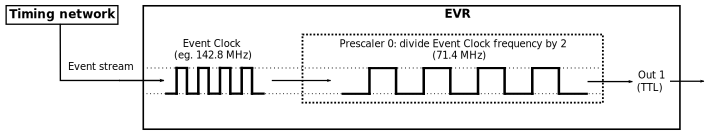
\includegraphics[width=\columnwidth]{./img/prescaler}
	\caption{An example clock signal generation}
	\label{fig:prescaler}
\end{figure}

\subsection{Instructions}
\begin{enumerate}
	\item If starting a new IOC application, consult the quick start in Section~\ref{sec:Quick start}.

	\item Set the macro values in the substitution file (\texttt{MTEST-VME-TIMINGTEST/} \texttt{cfg/EVR0.subs}) according to this snippet (explained in~\ref{sec:explain_clock}):
\begin{verbatim}
	file "$(mrfioc2_TEMPLATES=db)/evr-vme-230.db"
	{
	  {
	    ...
	    PS0-Div-SP=2,
	    ...
	    FrontOut1-Src-SP=40,
		    ...
	  }
	}
\end{verbatim}
	The above macro substitution of the \texttt{evr-vme-230.db} sets the values of the following records:
	\begin{itemize}
		\item \texttt{MTEST-VME-TIMINGTEST-EVR0:PS0-Div-SP}
		\item \texttt{MTEST-VME-TIMINGTEST-EVR0:FrontOut1-Src-SP}
	\end{itemize}
	
	\item Optionally, you can remove all the macros whose values you did not change. 
	\item Install the prepared IOC by running command \texttt{swit -V} from your project folder \textit{MTEST-VME-TIMINGTEST}.
\end{enumerate}

\subsection{Substitution snippet explanation:}\label{sec:explain_clock}
\begin{itemize}
	\item \texttt{PS0-Div-SP}=2: Set the Prescaler 0 to divide event clock frequency by 2.
	\item \texttt{FrontOut1-Src-SP}=40: Set the source of the Front Panel Output 1 to Prescaler 0. Values 40-42 correspond to prescalers 0-2. A complete list of values is available in the EVR manual~\cite{evr_manual}.
\end{itemize}

In order to use different prescaler, simply change the prescaler number, eg. using \texttt{PS2-Div-SP} instead of \texttt{PS0-Div-SP} sets the divider of prescaler 2 instead of prescaler 0.
Similar is for outputs, eg. using \texttt{FrontOut0-Src-SP} instead of \texttt{FrontOut1-Src-SP} sets the output source signal of front panel output 0 instead of front panel output 1.

\section{Generate the event clock}\label{sec:generate_event_clock}
Signals with frequency greater or equal to the frequency of the event clock can only be generated using the CML outputs. More about the operation of the CML outputs and their modes is available in the EVR manual~\cite{evr_manual}. Note, that not all event receiver form factors have CML outputs. The EVR-VME-230RF form factor has outputs FrontOut4 (CML0), FrontOut5 (CML1) and FrontOut6 (CML2) capable of CML output. This tutorial demonstrates how to configure CML0 output (corresponds to FrontOut4 output) to generate a clock signal, that has the same phase and frequency as the event clock. To achieve this, the FrontOut4 output source is set to \texttt{logic low} and the CML outputs are enabled. This causes the logic low pattern of the CML pulse mode to be continuously outputted. The configurable pattern, as seen in Figure~\ref{fig:gen_evt_clk}, is 20 bits long and is sent out with a bit rate of 20 times the event clock rate. It is configured to replicate the event clock phase and frequency.

\begin{figure}[H]
	\centering
	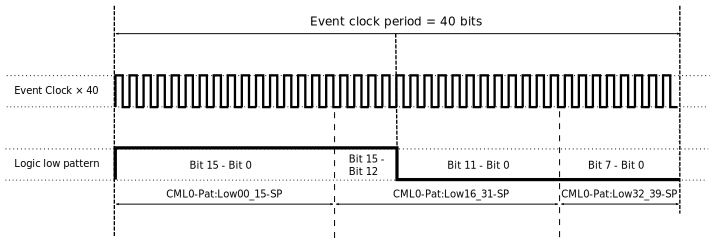
\includegraphics[width=\columnwidth]{./img/gen_evt_clk}
	\caption{Generate the event clock}
	\label{fig:gen_evt_clk}
\end{figure}

\subsection{Instructions}
\begin{enumerate}
	\item If starting a new IOC application, consult the quick start in Section~\ref{sec:Quick start}.
	
	\item Set the macro values in the substitution file (\texttt{MTEST-VME-TIMINGTEST/} \texttt{cfg/EVR0.subs}) according to this snippet (explained in~\ref{sec:explain_cml}):
\begin{verbatim}
	file "$(mrfioc2_TEMPLATES=db)/evr-vme-230.db"
	{
	  {
	    ...
	    FrontOut4-Ena-SP=1,
	    FrontOut4-Src-SP=63,
	    CML0-Ena-Sel=1,
	    CML0-Pwr-Sel=1,
	    CML0-Mode-Sel=0,
	    CML0-Pat:Low00_15-SP=0xFFC0,
	    CML0-Pat:Low16_31-SP=0, 
	    ...
	  }
	}
\end{verbatim}
	The above macro substitution of the \texttt{evr-vme-230.db} sets the values of the following records:
	\begin{itemize}
		\item \texttt{MTEST-VME-TIMINGTEST-EVR0:FrontOut4-Ena-SP}
		\item \texttt{MTEST-VME-TIMINGTEST-EVR0:FrontOut4-Src-SP}
		\item \texttt{MTEST-VME-TIMINGTEST-EVR0:CML0-Ena-Sel}
		\item \texttt{MTEST-VME-TIMINGTEST-EVR0:CML0-Pwr-Sel}
		\item \texttt{MTEST-VME-TIMINGTEST-EVR0:CML0-Mode-Sel}
		\item \texttt{MTEST-VME-TIMINGTEST-EVR0:CML0-Pat:Low00\_15-SP}
		\item \texttt{MTEST-VME-TIMINGTEST-EVR0:CML0-Pat:Low16\_31-SP}
	\end{itemize}

	\item Optionally, you can remove all the macros whose values you did not change. 
	\item Install the prepared IOC by running command \texttt{swit -V} from your project folder \textit{MTEST-VME-TIMINGTEST}.
\end{enumerate}

\subsection{Substitution snippet explanation:}\label{sec:explain_cml}
\begin{itemize}
	\item \texttt{FrontOut4-Ena-SP}=1: Enable the front panel output 4.
	\item \texttt{FrontOut4-Src-SP}=63: Set the source of the front panel output 4 to logic low. A complete list of settable values is available in the EVR manual~\cite{evr_manual}.
	\item \texttt{CML0-Ena-Sel}=1: Enable the CML0 output, which corresponds to the front panel output 4.
	\item \texttt{CML0-Pwr-Sel}=1: Power on the CML0 output.
	\item \texttt{CML0-Mode-Sel}=0: Select the pulse mode. Because the output source signal of the front panel output 4 is set to logic low, this mode will continuously output logic low pattern.
	\item \texttt{CML0-Pat:Low00\_15-SP}=0xFFC0: Set logic low pattern bits 0-15. The Figure~\ref{fig:gen_evt_clk} shows that the bits 15-0 must be set as follows: \texttt{1111 1111 1100 0000}, which translates to \texttt{0xFFC0}. Each bit represents $1/20$ of the event clock period.
	\item \texttt{CML0-Pat:Low16\_31-SP}=0: Set signal low pattern bits 16-31, as seen in Figure~\ref{fig:gen_evt_clk}. Note, that only bits 31-28 (top 4 bits) can be used.
\end{itemize}


\section{Output a Distributed Bus bit}
A custom distributed bus (DBus) bit can be outputted through desired EVR outputs. This tutorial demonstrates how to set up the DBus bit 0 as a source of an EVR front panel output 1, as seen in Figure~\ref{fig:dbus}. 
%To achieve this, the front panel output 0 should be mapped to the distributed bus bit (signal) 0. This is configured by setting the value of the output source macro \texttt{FrontOut1-Src-Sp} to 32. Mapping 32 corresponds to the DBus bit 0.

\begin{figure}[H]
	\centering
	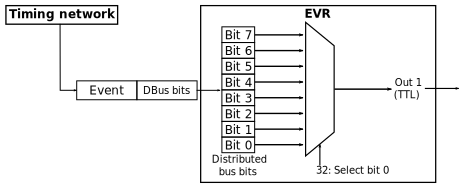
\includegraphics[]{./img/dbus}
	\caption{Send DBus bit 0 to the front panel output 1}
	\label{fig:dbus}
\end{figure}

\subsection{Instructions}
\begin{enumerate}
	\item If starting a new IOC application, consult the quick start in Section~\ref{sec:Quick start}.
	
	\item Set the macro values in the substitution file (\texttt{MTEST-VME-TIMINGTEST/} \texttt{cfg/EVR0.subs}) according to this snippet (explained in~\ref{sec:explain_dbus}):
\begin{verbatim}
	file "$(mrfioc2_TEMPLATES=db)/evr-vme-230.db"
	{
	  {
	    ...
	    FrontOut1-Src-SP=32,
	    ...
	  }
	}
\end{verbatim}
	The above macro substitution of the \texttt{evr-vme-230.db} sets the values of the following record:
	\begin{itemize}
		\item \texttt{MTEST-VME-TIMINGTEST-EVR0:FrontOut1-Src-SP}
	\end{itemize}

	\item Optionally, you can remove all the macros whose values you did not change. 
	\item Install the prepared IOC by running command \texttt{swit -V} from your project folder \textit{MTEST-VME-TIMINGTEST}.
\end{enumerate}

\subsection{Substitution snippet explanation:}\label{sec:explain_dbus}
\begin{itemize}
	\item \texttt{FrontOut1-Src-SP}=32: Set the source of the front panel output 1  to DBus bit 0. Values 32-39 correspond to DBus bits 0-7. A complete list of values is available in the EVR manual~\cite{evr_manual}.
\end{itemize}

In order to use different front panel output, simply change the front panel output number, eg. using \texttt{FrontOut0-Src-SP} instead of \texttt{FrontOut1-Src-SP} sets the output source signal of front panel output 0 instead of front panel output 1.

\section{Data buffer}\label{sec:data_buffer}
The timing system supports deterministic data transmission. Data buffer enables the event receivers to accept the transmitted data in a buffer. The data can be written and read from through EPICS records, which access the buffer in the EVR. In order to use this feature, \texttt{mrfioc2\_regDev} module~\cite{git_mrfioc2_regDev} must be loaded. For further details, inspect the readme file in the \texttt{mrfioc2\_regDev} git repository~\cite{git_mrfioc2_regDev}.


%When using the EVR as described in Section~\ref{sec:Quick start}, the following data/records are already available:
%\begin{itemize}
%\item Data regarding the beam synchronous readouts~\cite{bsread}:
%	\begin{itemize}
%	\item \texttt{\$(SYS)-\$(EVR):BunchIdRx-I}: The pulse ID,
%	\item \texttt{\$(SYS)-\$(EVR):BunchIdRx-MASTER-TS-SEC}: Seconds part of the pulse time-stamp,
%	\item \texttt{\$(SYS)-\$(EVR):BunchIdRx-MASTER-TS-NSEC}: Nanoseconds part of the pulse time-stamp,
%	\end{itemize}
%\end{itemize}
%where \texttt{\$(SYS)} is the system name (\textit{MTEST-VME-TIMINGTEST}) and \texttt{\$(EVR)} is the event receiver name (\textit{EVR0}).
%
%\begin{quote}
%\textbf{Adding data to the buffer should be coordinated with the entire team. Special care should be taken in order to avoid destroying existing data in the buffer.}
%\end{quote}
%
%The following instructions show how to use a combination of analogue in and analogue out records to read and write custom data in the data buffer:
%\begin{enumerate}
%\item If starting a new IOC application, consult the quick start in Section~\ref{sec:Quick start}.
%\item Create a new template file named \texttt{customData.template} with the following content in the project folder \textit{MTEST-VME-TIMINGTEST}:
%	\begin{verbatim}
%		record(ao, "$(SYS)-$(EVR):customData$(ID)-SP") {
%		  field(DTYP, "regDev")
%		  field(OUT, "@EVRDBUFF:$(OFFSET) T=double")
%		}
%		
%		record(ai, "$(SYS):$(EVR)-customData$(ID)-RB") {
%		  field(DTYP, "regDev")
%		  field(INP, "@EVRDBUFF:$(OFFSET) T=double")
%		  field(SCAN, "I/O Intr")
%		}
%	\end{verbatim}
%	The \texttt{\$(SYS)-\$(EVR):customData\$(ID)-SP} record is used to write the data at the specified offset in the data buffer. Once the data is written, it can be read from any EVR in the timing system, which has the %counterpart \texttt{\$(SYS):\$(EVR)-customData\$(ID)-RB} record (an analogue in record with the same offset).
%	\begin{itemize}
%		\item 
%			\texttt{\$(SYS)} is the system name, and \texttt{\$(EVR)} is the event receiver name. The \texttt{\$(ID)} is a unique identification of the record.
%		\item 
%			In order to use records for reading and writing data to the data buffer, device type must be set to \texttt{regDev}~\cite{regDev}.
%		\item 
%			\texttt{INP} and \texttt{OUT} fields of the record specify the type of the data (\texttt{T=double}), the buffer name and the buffer offset(\texttt{\$(OFFSET)}) to read/write. When using the EVR as described in %Section~\ref{sec:Quick start}, the buffer name is always \texttt{EVRDBUFF}. Offset is in range of \texttt{0x04 - 0x7FC} bytes.
%		\item 
%			When new data is available to read, an interrupt is fired. The \texttt{\$(SYS):\$(EVR)-customData\$(ID)-RB} record gets processed on each interrupt (\texttt{field(SCAN, "I/O Intr")}), thus the record's value is updated %with the new data.
%	\end{itemize}
%
%\item Add the following to the \texttt{MTEST-VME-TIMINGTEST\_main.subs} file:
%	\begin{verbatim}
%	file "customData.template"{
%	pattern {  SYS,                    EVR,    ID, OFFSET }
%	        { "MTEST-VME-TIMINGTEST",    "EVR0",  0,  0x50}
%	        { "MTEST-VME-TIMINGTEST",    "EVR0",  1,  0x60}
%	}
%	\end{verbatim}
%	The above substitution creates the following records:
%	\begin{itemize}
%		\item \texttt{MTEST-VME-TIMINGTEST:EVR0-customData0-SP}: Used to write a value of type double to buffer offset \texttt{0x50}.
%		\item \texttt{MTEST-VME-TIMINGTEST:EVR0-customData1-SP}: Used to write a value of type double to buffer offset \texttt{0x60}.
%		\item \texttt{MTEST-VME-TIMINGTEST:EVR0-customData0-RB}: Used to read a value of type double from the buffer offset \texttt{0x50}
%		\item \texttt{MTEST-VME-TIMINGTEST:EVR0-customData1-RB}: Used to read a value of type double from the buffer offset \texttt{0x60}
%	\end{itemize}
%\item Install the prepared IOC by running command \texttt{swit -V} from your project folder \textit{MTEST-VME-TIMINGTEST}.
%\end{enumerate}

\section{Advanced: Trigger switching between normal and off beam operation}\label{sec:triggerSwitching}
\begin{quote}
\textbf{This functionality is only available on event receivers that support pulser gating (eg. EVR-VME-300 series)!}
\end{quote}

This tutorial is the advanced version of tutorial in Section~\ref{sec:2pulsers}. It demonstrates the same configuration without using \texttt{evr-configTriggerSwitch.template} helper template.

Often devices need to be triggered with a different delay, based on the status of the beam or machine protection system (MPS). This status is available on the event receiver as presence or absence of an event. In SwissFEL setup, there is an event called \texttt{RF OFF beam}, that is present:
\begin{itemize}
\item when MPS is asserted and
\item when RF is configured to not generate a beam (controlled by \texttt{RF ON} frequency set in the Timing master application, which is responsible for calculation of events to be emitted on the timing network).
\end{itemize}
\texttt{RF OFF beam} event can thus be used as an indication weather a device should be triggered with a delay or not.

Event receivers that support pulser gating also support setting two sources to one physical output. These functionalities can be used to set up two pulsers with different settings (eg. different delays) and select which pulse will be outputted based on the presence of an event (eg. \texttt{RF OFF beam}). Configuring such behavior involves the following steps:
\begin{enumerate}
\item Select two pulsers (eg. Pulser 22 and Pulser 23) and set them as output sources for desired physical output (eg. FrontUnivOut0). \label{mps_steps:selectPulsers}
\item Configure the first pulser (eg. set pulse width and delay) for normal device operation (eg. when \texttt{RF OFF beam} is not present). \label{mps_steps:configurePulser1}
\item Configure the second pulser (eg. set pulse width and delay) for off-beam device operation (eg. when \texttt{RF OFF beam} is present). \label{mps_steps:configurePulser2}
\item Define desired event number to trigger both pulsers.  \label{mps_steps:triggerEvent}
\item Configure pulser gate (eg. pulser 28 which represents gate 0) to be set by off-beam event (eg. \texttt{RF OFF beam}) and reset by start of sequence event (\texttt{SOS}). \label{mps_steps:setupGate}
\item Set first pulser to be masked by pulser gate (eg. pulser 28 = pulser gate 0 = mask 0x01). \label{mps_steps:setPulserMask}
\item Set second pulser to be enabled by pulser gate (eg. pulser 28 = pulser gate 0 = enable 0x01). \label{mps_steps:setPulserEnable}
\end{enumerate}
For more information about pulser gating and outputs with two configurable sources inspect the EVR manual~\cite{evr_manual}.

This tutorial demonstrates how to configure an EVR without using helper template to:
\begin{itemize}
\item generate a 40~ns wide pulse, 40~ns after each reception of event 4 in normal operation (when \texttt{RF OFF beam} is not present).
\item generate a 40~ns wide pulse, 80~ns after each reception of event 4 in off-beam operation (when \texttt{RF OFF beam} is present).
\item The pulse is outputted through front panel universal TTL output 0 (FrontUnivOut0).
\end{itemize}
%The setup is depicted in Figure~\ref{fig:2pulsers}.

\subsection{Instructions}\label{sec:instructions_triggerSwitching}
\begin{enumerate}
	\item If starting a new IOC application, consult the quick start in Section~\ref{sec:Quick start}, but use the substitution file at \texttt{https://git.psi.ch/epics\_drivers/}\newline \texttt{mrfioc2/raw/\latestDriverVersion/PSI/example/evr\_VME-300.subs} in step~\ref{quickstart:copySubs}. 

	\item \label{sec:gating_instructions1_setMacro} Set the macro values in the substitution file (\texttt{MTEST-VME-TIMINGTEST/} \texttt{cfg/EVR0.subs}) according to this snippet (explained in~\ref{sec:explain_triggerSwitching}):
\begin{verbatim}
	file "$(mrfioc2_TEMPLATES=db)/evr-vme-300.db"
	{
	  {
	    ...
	    Pul22-Delay-SP=40,
	    Pul22-Width-SP=40,
	    Pul22-Gate-Mask-SP=0x1,
	    ...
	    Pul23-Delay-SP=80,
	    Pul23-Width-SP=40,
	    Pul23-Gate-Enable-SP=0x1,
	    ...
	    FrontUnivOut0-Src-SP=22,
	    FrontUnivOut0-Src2-SP=23,
	    ...
	  }
	}

	file "$(mrfioc2_TEMPLATES=db)/evr-pulserMap.template"{
	pattern { PID   F,       EVT, ID}
	        ...
	        { 22,   Trig,    4,   0 }
	        { 23,   Trig,    4,   0 }
	        ...
	        { 28,   Set,     6,   0 }
	        { 28,   Reset,   40,  0 }
	        ...
	}
\end{verbatim}
	The above macro substitution of the \texttt{evr-vme-300.db} sets the values of the following records:
	\begin{itemize}
		\item \texttt{MTEST-VME-TIMINGTEST-EVR0:Pul22-Delay-SP}
		\item \texttt{MTEST-VME-TIMINGTEST-EVR0:Pul22-Width-SP}
		\item \texttt{MTEST-VME-TIMINGTEST-EVR0:Pul22-Gate-Mask-SP}
		\item \texttt{MTEST-VME-TIMINGTEST-EVR0:Pul23-Delay-SP}
		\item \texttt{MTEST-VME-TIMINGTEST-EVR0:Pul23-Width-SP}
		\item \texttt{MTEST-VME-TIMINGTEST-EVR0:Pul23-Gate-Enable-SP}
		\item \texttt{MTEST-VME-TIMINGTEST-EVR0:FrontUnivOut0-Src-SP}
		\item \texttt{MTEST-VME-TIMINGTEST-EVR0:FrontUnivOut0-Src2-SP}
	\end{itemize}
	The above macro substitution of the \texttt{evr-pulserMap.template} creates records named \texttt{MTEST-VME-TIMINGTEST-EVR0:Pul\$(PID)-Evt-\$(F)\$(ID)-SP}. In this case the record names are:
	\begin{itemize}
		\item \texttt{MTEST-VME-TIMINGTEST-EVR0:Pul22-Evt-Trig0-SP}
		\item \texttt{MTEST-VME-TIMINGTEST-EVR0:Pul22-Evt-Trig0-SP}
		\item \texttt{MTEST-VME-TIMINGTEST-EVR0:Pul28-Evt-Set0-SP}
		\item \texttt{MTEST-VME-TIMINGTEST-EVR0:Pul28-Evt-Reset0-SP}
	\end{itemize}
	
	\item Optionally, you can remove all the macros whose values you did not change. 
	\item Install the prepared IOC by running command \texttt{swit -V} from your project folder \textit{MTEST-VME-TIMINGTEST}.
\end{enumerate}

\subsection{Substitution snippet explanation:}\label{sec:explain_triggerSwitching}

First we set up the pulse generator 22 (Pul22) and  pulse generator 23 (Pul23).
\begin{itemize}
	\item \texttt{Pul22-Delay-SP}=40: Set the delay between the reception of the event and the start of the pulse (pulse rising edge) for pulser 22 to 40 ns. 
	\item \texttt{Pul22-Width-SP}=40: Set the pulse width (time between the pulse rising and falling edge) for pulser 22 to 40 ns.
	\item \texttt{Pul23-Delay-SP}=80: Set the delay between the reception of the event and the start of the pulse (pulse rising edge) for pulser 23 to 80 ns. 
	\item \texttt{Pul23-Width-SP}=40: Set the pulse width (time between the pulse rising and falling edge) for pulser 23 to 40 ns.
	\item \texttt{Pul22-Gate-Mask-SP}=0x1: Set the gate 0 to mask pulser 22. While the selected gate is activated, this pulser's \textit{Trig} function is inhibited. Gates are selected using a bit mask, eg. value 0x1 corresponds to gate 0.
	\item \texttt{Pul23-Gate-Enable-SP}=0x1: Set the gate 0 to enable this pulser. While the selected gate is not activated, this pulser's \textit{Trig} function is inhibited. Gates are selected using a bit mask, eg. value 0x1 corresponds to gate 0.
\end{itemize}

Then, the value of the output source macros \texttt{FrontUnivOut0-Src-SP} and \texttt{FrontUnivOut0-Src2-SP} is set to 22 and 23 respectively, which configures the front panel output 0 (FrontUnivOut0) to use pulsers 22 and 23 as its source. Macro values 0-23 correspond to pulsers 0-23. A complete list of available values can be found in the EVR manual~\cite{evr_manual}.

Pulser 22 and Pulser 23 are then set to trigger on reception of the event 4:
\begin{itemize}
	\item \texttt{PID}: Select Pulser 22/23
	\item \texttt{F}: Select the \textit{Trig} (trigger) function of the pulser
	\item \texttt{EVT}: Map Pulser 22/23 \textit{Trig} function to event 4
	\item \texttt{ID}: Unique ID for each PID-F combination.
\end{itemize}

Finally, Pulser 28, which represent pulser gate 0, is configured to be set upon reception of \texttt{RF OFF beam} event (event code 6), and reset upon reception of \texttt{SOS} event (event code 40):
\begin{itemize}
	\item \texttt{PID}: Select Pulser 28 (pulser gate 0)
	\item \texttt{F}: Select the \textit{Set} and \textit{Reset} function of the pulser
	\item \texttt{EVT}: Map Pulser 28 \textit{Set} function to event 6 and \textit{Reset} function to event 40.
	\item \texttt{ID}: Unique ID for each PID-F combination.
\end{itemize}

In order to use different pulser, simply change the pulser number, eg. using \texttt{Pul20-Delay-SP} instead of \texttt{Pul22-Delay-SP} sets the delay of pulser 20 instead of pulser 22.

Similar is for outputs, eg. using \texttt{RearUniv0-Src-SP} and \texttt{RearUniv0-Src2-SP} instead of \texttt{FrontUnivOut0-Src-SP} and \texttt{FrontUnivOut0-Src2-SP} sets the output source signal of rear panel output 1 instead of front panel output 0. 

In order to set a different event mapped to Pulsers 22 and 23 Trig function, simply set a new value of records \texttt{MTEST-VME-TIMINGTEST-EVR0:Pul22-Evt-Trig0-SP} and \texttt{MTEST-VME-TIMINGTEST-EVR0:Pul23-Evt-Trig0-SP}. To disable the mapping, set records value to \texttt{0}.

Similar is for changing events that set and reset the pulser gate. In order to set a different event mapped to setting the gate (which controls when off-beam operation is in affect), simply set a new value of the \newline\texttt{MTEST-VME-TIMINGTEST-EVR0:Pul28-Evt-Set0-SP} record.


\section{GUI}\label{sec:gui} 
There is a caQtDM~\cite{caqtdm} GUI for the Event Receiver available. It can be used to further configure the EVR or simply check the running configuration. The GUI is launched using the following command:

\begin{verbatim}
	start_EVR.sh -s <system name> [options]
\end{verbatim}
where the \texttt{<system name>} represents a \textbf{mandatory} system name, and \texttt{[options]} are as follows:
\begin{verbatim}
	-d <EVR name> ......... set the event receiver / timing card name 
	                        (default:EVR0)
	-f <form factor> ...... choose the event receiver form factor 
	                        (default: VME-300)
	                        Choices: VME, PCIe, VME-300
	-h    ................. shows the options and usage
\end{verbatim}


\paragraph{Example 1:} Open the GUI for the EVR-VME-300 event receiver named \texttt{EVR0}, using system name \texttt{MTEST-VME-TIMINGTEST}.
\begin{verbatim}
	start_EVR.sh -s MTEST-VME-TIMINGTEST
\end{verbatim}

\paragraph{Example 2:} Open the GUI for the EVR-VME-230RF event receiver named \texttt{EVR3}, using system name \texttt{MTEST-VME-TIMINGTEST}.
\begin{verbatim}
	start_EVR.sh -s MTEST-VME-TIMINGTEST -d EVR3
\end{verbatim}

\paragraph{Example 2:} Open the GUI for the EVR-PCIe-300 event receiver named \texttt{EVR0}, using system name \texttt{MTEST-VME-TIMINGTEST}.
\begin{verbatim}
	start_EVR.sh -s MTEST-VME-TIMINGTEST -f PCIe
\end{verbatim}

\paragraph{Example 3:} Shows options and usage.
\begin{verbatim}
	start_EVR.sh -h
\end{verbatim}

\bibliographystyle{plain}
\bibliography{references}
%\printbibliography

\end{document}
